% illustrer les performances ainsi que l'efficacité du logiciel implémenté
% a l'aide de graphiques.


% analyser (et comparer, si plusieurs) les performances des solutions 
% implémentées


% présenter les bancs d'essais (ou les procédures utilisées pour la génération)
% des données) utilisés pour les tests du logiciel.

\section{Observations de l'algorithme MinMax sur nos jeux}
Une fois l'implémentation de l'algorithme \emph{MinMax} faite sur nos deux
jeux combinatoires, nous pouvons nous demander, est-ce que cet algorithme est adapté pour le jeu de Hex et de l'Awalé ?
Nous observons que les performances du \emph{MinMax} sont très différentes d'un jeu à l'autre. Dans cette section nous étudierons ces différences.

\subsection{Hexgame : Performances décevantes}
L'algorithme \emph{MinMax} développé sur le jeu du Hex n'arrive quasiment jamais à battre un humain, et cela, pour
deux raisons principales : la faible profondeur, et la difficulté à trouver une fonction d'évaluation satisfaisante.

\paragraph{Trop grande complexité} Le premier problème provient du nombre de coups possibles à chaque tour.
En effet, sur un plateau classique de $13\times13$ le premier joueur a 169 coups possibles. Au coup suivant, il y en a 168 etc\dots Cela rend les calculs lents. 
Si l'ordinateur joue en premier, et que la profondeur de calcul est de 6, celui-ci doit calculer pas moins de $2.1298467e+13$ (soit $169\times168\times167\times166\times165\times164$)
fois la fonction d'évaluation. Cela n'est pas réalisable en temps réaliste. Dans notre implémentation, la taille des côtés du plateau varie entre
une longueur de 5 cases et de 17. Nous avons remarqué que pour un plateau de dimension $11\times11$, et une profondeur demandée de 4, l'algorithme
mettait déjà plusieurs secondes à calculer le meilleur coup. Notons que ces calculs ne prennent pas en compte l'élagage alpha-bêta
qui optimise significativement le \emph{MinMax}. Même si une portion des nœuds n'est pas évaluée, le calcul reste trop lent pour pouvoir demander une
profondeur plus intéressante de 6 ou de 8 par exemple.
On peut aussi noter que la performance de l'élagage alpha-bêta dépend de la qualité de la fonction d'évaluation, qui, comme nous allons
le voir, n'est pas assurée.

\paragraph{Fonction d'évaluation : Un vrai casse-tête}
Le \emph{MinMax} n'arrivant pratiquement jamais à une feuille terminale, nous avons compris que la fonction
d'évaluation du Hex devait être performante et peu coûteuse en temps. Cependant, faire comprendre à l'ordinateur si une position est gagnante
ou non s'est révélé très difficile. En effet, le Hex est un jeu possédant de nombreuses stratégies, et relier toutes ces stratégies en une
seule fonction d'évaluation n'est pas chose aisée. Ainsi, nous avons rapidement cherché à faire comprendre à l'ordinateur
quelle stratégie adapter au fur et à mesure de la partie. Parmi elles, la stratégie de faire des ponts (voir la figure 3) nous a posé beaucoup de problèmes.
Un pont permet au joueur de s'assurer de pouvoir connecter deux pièces lors d'un prochain coup. En effet, si le joueur adversaire cherche à bloquer
l'une des deux cases, nous avons juste à ajouter notre jeton afin de créer un chemin entre ces deux pièces. Nous pouvons noter que lorsque la profondeur de
réflexion du \emph{MinMax} est grande, il arrive parfois à remarquer que créer un pont est le meilleur coup. Mais nous revenons au problème n°1 : la complexité.
Voir la section sur les fonctions d'évaluations pour voir quelles idées nous avons essayé. Notre fonction finale est capable de battre des humains sur de petits 
plateaux. Mais en général, lorsque le plateau est de grande dimension, la fonction d'évaluation prend de nombreuses secondes, voire minutes avant de jouer.

\begin{figure}[h]
    \begin{center}
        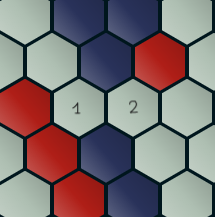
\includegraphics[scale=0.5]{root/pont.png}
    \end{center}
    \caption[1]{Ici bleu a créé un pont\footnotemark.}\label{fig:pont_bleu}
\end{figure}

\footnotetext{Si rouge joue sur la case 1, bleu joue sur la case 2, et relie ainsi les deux jetons bleus (respectivement si rouge joue sur la case 2)}



\subsection{Awalé : Bonnes performances}
\paragraph{Une fonction d'évaluation efficace} 
Le jeu de l'Awalé possède un avantage significatif par rapport au Hex, le nombre maximum de coups
possible pour un joueur est de 6. Ainsi, l'arbre de recherche est bien plus petit que celui du Hex. L'algorithme \emph{MinMax} est donc efficace en termes de
temps et de performances avec une grande profondeur (la profondeur initiale est de 6 ou 8).

Le choix de notre fonction d'évaluation est arrivé naturellement pendant nos recherches. Nous avons implémenté la simple fonction cherchant à
maximiser les points de l'ordinateur tout en minimisant les points de son adversaire. Cette fonction combinée à une profondeur de taille 6 en fait un
adversaire redoutable que peu d'humains ont réussi à battre.

\subsection{Conclusion}
L'algorithme \emph{MinMax} est donc capable d'être efficace lorsque le nombre de nœuds est petit à chaque itération. On peut alors
lui mettre une profondeur relativement grande afin d'explorer toutes les branches de cet arbre.
Cependant, lorsque le nombre de nœuds devient gigantesque, comme dans le Hex, l'algorithme ne devient plus très bon. Il est en effet très lent et peu performant.
Dans la bibliographie est disponible un lien vers un papier scientifique cherchant une bonne fonction d'évaluation pour le Hex.
Dans celui-ci, il est écrit que les ordinateurs battent les humains pour des petits plateaux, font jeu égal pour le plateau 9x9 mais
sont moins bons qu'un humain pour un plus grand plateau. On y voit aussi la difficulté de trouver une bonne fonction d'évaluation.
